\chapter{Evaluation}\label{chap:evaluation}
The contribution of this thesis is the direct comparison of the network architectures presented in the previous section on data from the Business Process Intelligence Competitions 2011 and 2012~\cite{BPIC2011, BPIC2012}. The execution of this comparison in code, the preceding data preparation and transformation as well as the obtained results shall be presented in this chapter.

\section{Implementation}
Anaconda~\cite{web:anaconda} was set up to create a stable working environment in which dependencies and libraries would not change.
Then, the data was explored, prepared and cleansed in an iterative fashion using JupyterLab notebooks~\cite{web:jupyter}. Helpful libraries in the process were prefixspan-py~\cite{web:prefixspan-py} and OpyenXes~\cite{web:opyenxes}. These notebooks were also used to develop the ANN training code in Keras~\cite{web:keras}.

As the codebase became more mature, Docker containers were built with the Anaconda environment inside them~\cite{web:docker}. Using a version of Docker for GPU applications running on NVIDIA hardware~\cite{web:nvidia-docker}, the networks were trained on the GPU cluster infrastructure of the HPI FutureSOC Lab~\cite{web:fsoc}.
The source code used in this thesis is available for download at: \url{https://github.com/flxw/master-thesis-code}.

\section{Data preprocessing}
Following the KDD process~\cite{fayyad1996data}, the data was preprocessed to eliminate generally known properties that hinder machine learning model performance. Here, this encompassed two steps for both datasets:

\begin{enumerate}
    \item All columns which exhibited zero entropy, i.e. were constituted of a single value, were dropped
    \item Using the bias-corrected version of Cramér's~V~\cite{bergsma2013bias}, features that correlate strongly were dropped
\end{enumerate}


For both BPIC2011 and BPIC2012 datasets, the column \texttt{lifecycle:transition} was dropped in step 1. To make statements about upcoming workflow-related activities only, only completion events related to workflow activities were kept in the BPIC2012 log \cite{evermann2016}.

In step 2, the bi-directional results in \autoref{fig:bpic2011-correlation-heatmap} from Cramér's V revealed that the variables \texttt{Producer code}, \texttt{Activity code} and \texttt{Specialism code} correlated strongly with many others in the BPIC2011 dataset. Thus, these were dropped.

As evidenced in \autoref{fig:bpic2012-correlation-heatmap}, the BPIC2012 dataset with its small number of features did not require any removals.

\begin{figure}
\centering
\subfloat[][BPIC2011 Cramér's V heatmap]{
    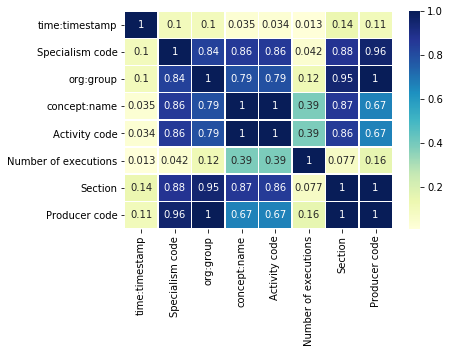
\includegraphics[width=0.4\textwidth]{gfx/bpic2011-correlation-matrix.png}
    \label{fig:bpic2011-correlation-heatmap}
}
\qquad
\subfloat[][BPIC2012 Cramér's V heatmap]{
    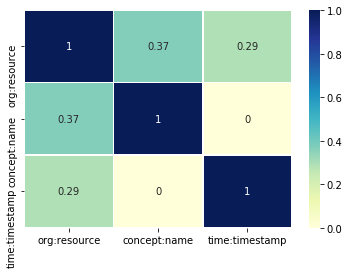
\includegraphics[width=0.4\textwidth]{gfx/bpic2012-correlation-matrix.png}
    \label{fig:bpic2012-correlation-heatmap}
}
\caption{Correlation heatmaps generated from the application of Cramér's V.}
\end{figure}

\section{Data transformation}
Having removed unneeded features, the remaining ones were encoded following standard practice. All numerical features $x$ were normalized individually for every trace using the well-tested min-max method:

$$z = \frac{x-min(x)}{max(x)-min(x)}$$

Categorical features without ordinal properties, which were all of them, were encoded using one-hot encoding if possible. In the case of the input for Evermann's model, they were encoded with dictionary encoding, as this encoding is required for Embedding layers.

\subsection*{SP-2 feature engineering}
The SP-2 features for the SP2 model were engineered in an iterative fashion, as \autoref{lst:sp2-generation} outlines. For every trace, a new data frame \texttt{sp2\_df} is created and the occurence of the first activity is marked inside it. For all following activities, the contents of the previous row inside \texttt{sp2\_df} are copied into the current one and the presence of the current activity is marked. This repeats itself until the trace has been iterated over.

\begin{lstlisting}[caption={SP-2 feature generation algorithm for a single trace},label={lst:sp2-generation}]
sp2_df = pd.DataFrame(columns=activity_labels, index=range(0,len(t)), dtype=np.bool)
for col in sp2_df.columns: sp2_df[col].values[:] = 0
sp2_df["{0}{1}".format(sp2_prefix, t["concept:name"][0])].values[0]  = 1

for i in range(1,len(t)):
    first_activity_name = t["concept:name"].iloc[i]
    col = "{0}{1}".format(sp2_prefix,first_activity_name)
    
    sp2_df.values[i] = sp2_df.values[i-1]
    sp2_df[col].values[i] = 1
\end{lstlisting}

\subsection*{Sub-sequence feature engineering}
The sub-sequence features for the PFS model were created with the help of the \textit{prefixspan-py} library~\cite{web:prefixspan-py}.

\begin{lstlisting}
# Prefixspan requires an array of arrays with one subarray for every trace
encoded_traces = [ t[target_column].map(feature_dict[target_column]['to_int']).tolist() for t in traces ]
prefixspan_traces = PrefixSpan(encoded_traces)
closed_sequences = prefixspan_traces.topk(25, closed=True) # support is how often the subsequence appears in total
# http://sequenceanalysis.github.io/slides/analyzing_sequential_user_behavior_part2.pdf, slide 5

# only take subsequence which are at a certain level of support? like if ss[0]/len(traces) < .90
#ps_topkc = list(filter(lambda x: x[0]/len(traces) > .90, ps_topkc))
closed_sequences = [ p[1] for p in closed_sequences ]
pftrace_args = [ (t, closed_sequences[:], feature_dict[target_column]['to_int']) for t in traces ] # enrich traces with copy of mined subsequences
\end{lstlisting}

\begin{lstlisting}
def enrich_trace_with_subseq(t, ps, event_to_int):
    col_prefix = "PFS_"
    subseq_labels = [ "{0}{1}".format(col_prefix,ss_idx) for ss_idx, ss in enumerate(ps) ]
    subseq_df = pd.DataFrame(columns=subseq_labels, index=range(0,len(t)), dtype=np.bool)
    
    for col in subseq_df.columns: subseq_df[col].values[:] = 0
    for i in range(0,len(t)): # loop through sequence, prune items from mined sequences, and once a subsequence array is empty, this subsequence has occured :)
        activity_code = event_to_int.get(t["concept:name"].iloc[i], None)
        
        for subseq_idx in range(0,len(ps)):
            if ps[subseq_idx] == []:
                continue
            if ps[subseq_idx][0] == activity_code:
                ps[subseq_idx].pop(0)
                if ps[subseq_idx] == []:
                    subseq_df.values[i:,subseq_idx] = 1
        
    return subseq_df
\end{lstlisting}

\section{Test setup}
Dropping the embedding layer if results are really bad
Iterative way of working
Making embedding layer optional
How batches, timesteps and samples were framed for this problem

\section{Results}
Three metrics of the four aforementioned implementations shall be the focus of the evaluation of the results:
\begin{enumerate}
    \item\textbf{Accuracy} - I.e. how many next-activity predictions were correct in total.
    \item\textbf{Earliness} - I.e. whether and how early in the total trace the prediction accuracy begins to stabilize \cite{francescomarino2015}.
    \item\textbf{Feature importance} - I.e. whether network-internal metrics indicate that an added feature is valuable for making predictions.
\end{enumerate}

Accuracy and earliness

Does accuracy rise with increasing trace length?
Feature Importance score extraction

\section{Discussion}
Is the hassle worth it?
Increase in memory, training time...?
Compare with Evermanns etc results